\documentclass[14pt,a4paper]{scrartcl}
\usepackage[left=0.1cm,right=0.1cm,
    top=0.1cm,bottom=0.1cm,bindingoffset=0cm]{geometry}

\usepackage[T1,T2A]{fontenc}
\usepackage[utf8]{inputenc}
\usepackage[english,russian,ukrainian]{babel}
\usepackage{tabularx}
\usepackage{amssymb}
\usepackage{color}
\usepackage{amsmath}
\usepackage{mathrsfs}
\usepackage{listings}
\usepackage{graphicx}
\graphicspath{ {./images/} }
%\usepackage{draftwatermark} не будет лезть на картинки
\usepackage[printwatermark]{xwatermark}%будет лезть на картинки
\usepackage{lipsum}
\usepackage{xcolor}
\begin{document}
\pagestyle{plain}
\pagecolor{white}
















\begin{figure}[h]
\center{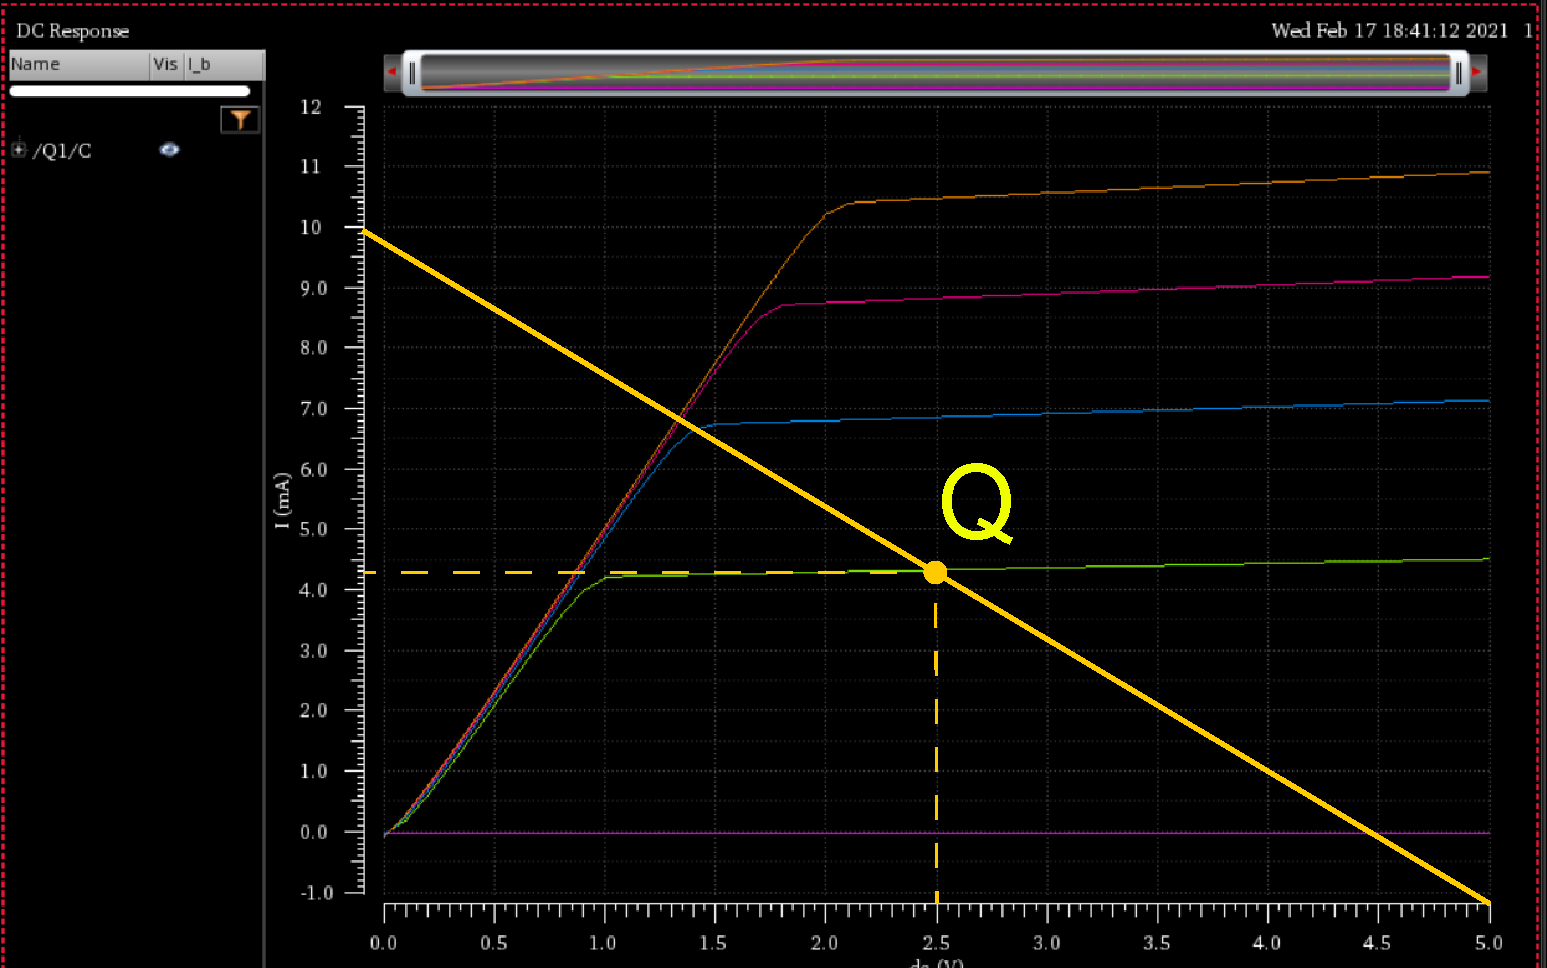
\includegraphics[width=27 cm, height = 19 cm, angle=270]{1.jpg} }
\end{figure}

\begin{figure}[h]
\center{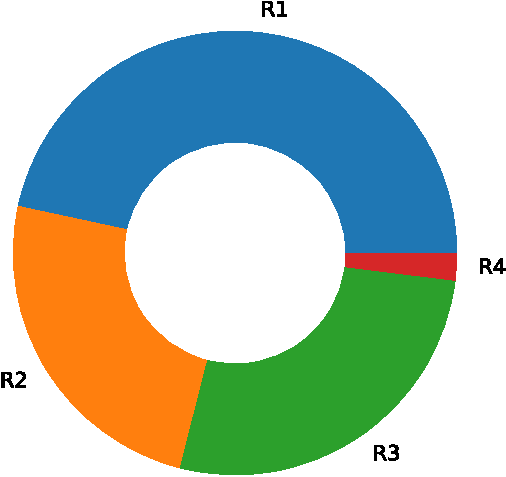
\includegraphics[width=27 cm, height = 19 cm, angle=270]{2.jpg} }
\end{figure}
\begin{figure}[h]
\center{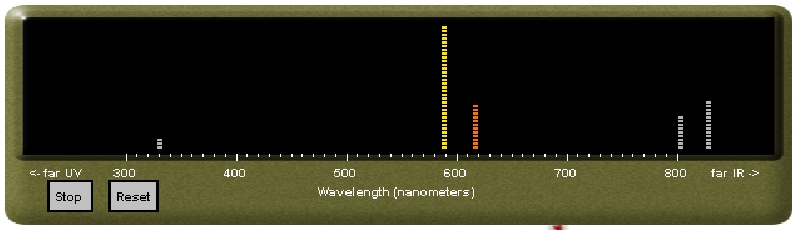
\includegraphics[width=27 cm, height = 19 cm, angle=270]{3.jpg} }
\end{figure}
\begin{figure}[h]
\center{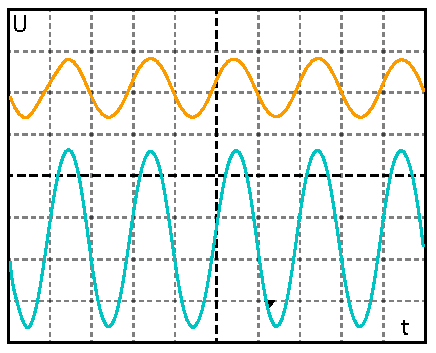
\includegraphics[width=27 cm, height = 19 cm, angle=270]{4.jpg} }
\end{figure}
\begin{figure}[h]
\center{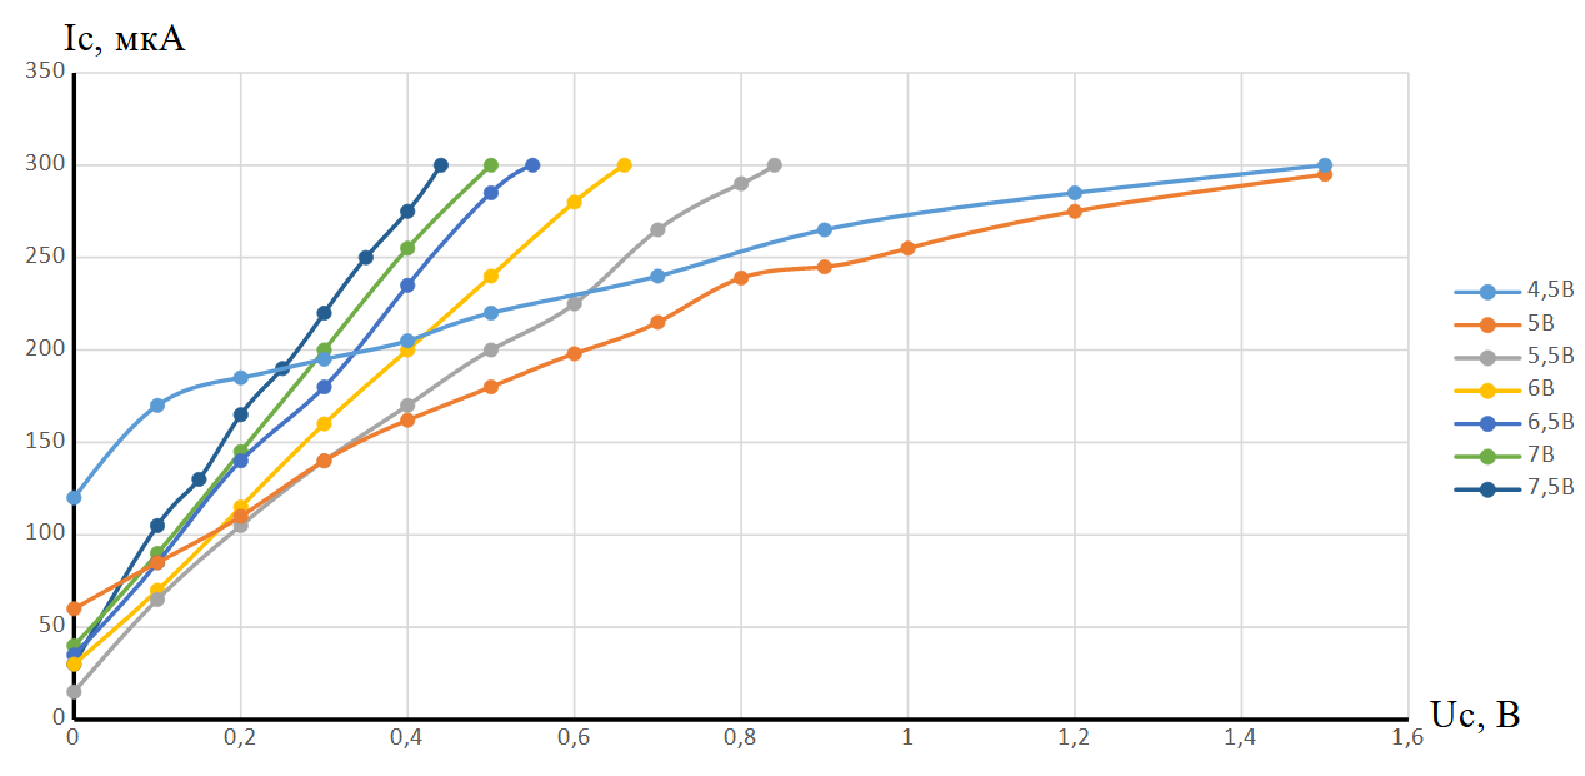
\includegraphics[width=27 cm, height = 19 cm, angle=270]{5.jpg} }
\end{figure}
\begin{figure}[h]
\center{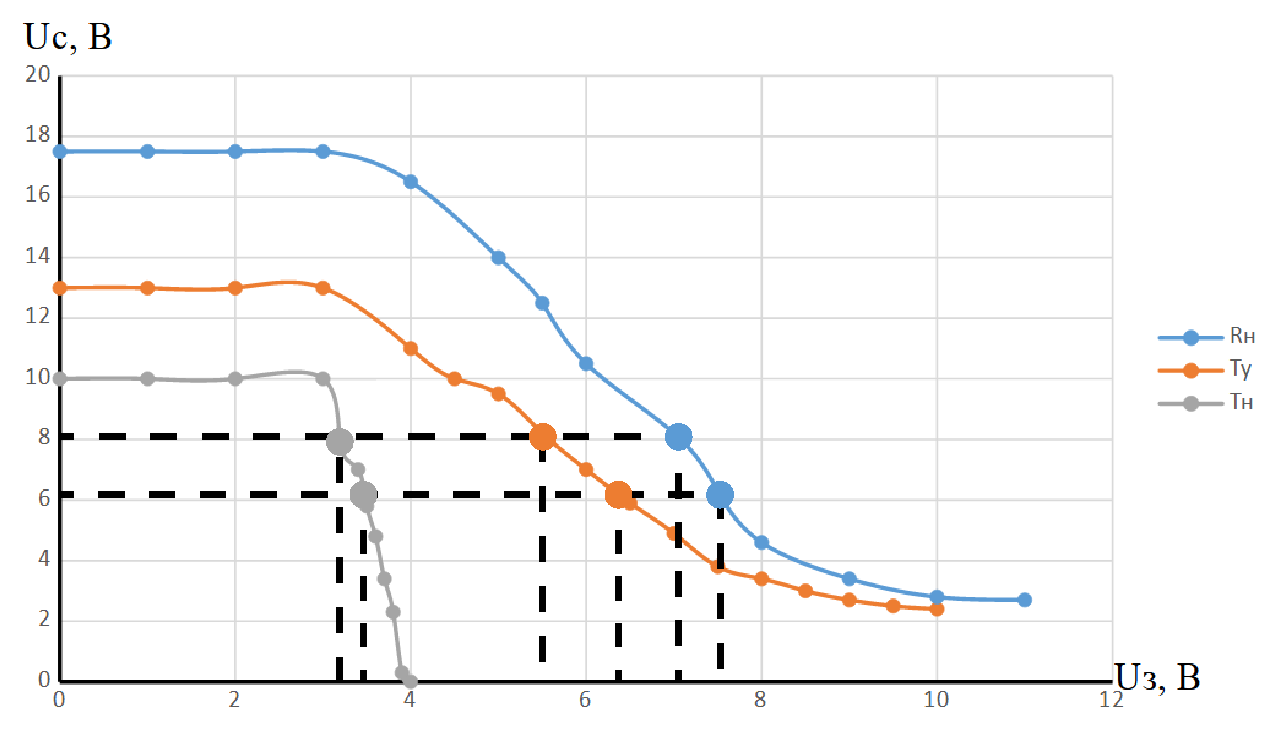
\includegraphics[width=27 cm, height = 19 cm, angle=270]{6.jpg} }
\end{figure}
\begin{figure}[h]
\center{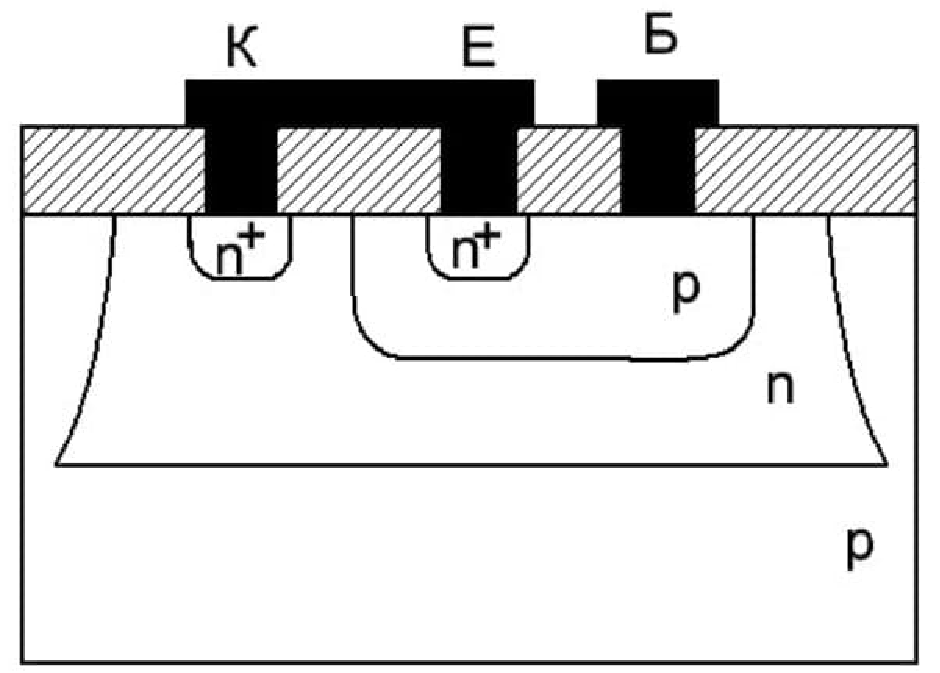
\includegraphics[width=27 cm, height = 19 cm, angle=270]{7.jpg} }
\end{figure}


















\end{document}